\documentclass{article}

\usepackage[utf8x]{inputenc}
\usepackage[english,russian]{babel}
\usepackage{cmap}
\usepackage{commath}
\usepackage{amsmath}
\usepackage{amsfonts}
\usepackage{mathtools}
\usepackage{amssymb}
\usepackage{parskip}
\usepackage{titling}
\usepackage{color}
\usepackage{hyperref}
\usepackage{cancel}
\usepackage{enumerate}
\usepackage{multicol}
\usepackage{graphicx}
\usepackage[font=small,labelfont=bf]{caption}
\usepackage[a4paper, left=2.5cm, right=1.5cm, top=2.5cm, bottom=2.5cm]{geometry}

\graphicspath{ {./images/} }
\setlength{\droptitle}{-3cm}
\hypersetup{ colorlinks=true, linktoc=all, linkcolor=blue }
\pagenumbering{arabic}

\begin{document}
    \textbf{5. Графический способ задания функции}
    
    \textbf{Определение 1.} Пусть на плоскости $\textrm{П}$ задана прямоугольная система координат и функция $f:\ A \rightarrow B$. Графиком $\textrm{Г}_f$ называется множество точек $(x, y)$ плоскости $\textrm{П}$, таких что $x \in A$, $y = f(x)$.
    \[\textrm{Г}_f \{ (x,\ f(x)) \in \textrm{П},\ x \in A\}\]
    В основном мы видим всего лишь приближение, а не график. Есть функции, график которой нельзя построить.

    \textbf{Пример.}

    1) Функция Дирихле. $D(x) = \begin{cases}
        1, & x \in \mathbb{Q}\\
        0, & x \not\in \mathbb{Q}
    \end{cases}$

    2) Функция Сигнум. $sign(x) = \begin{cases}
        1, & x > 0\\
        0, & x = 0\\
        -1, & x < 0
    \end{cases}$

    3) Функция модуля. $f(x) = \abs{x} = \begin{cases}
        x, & x > 0\\
        0, & x = 0\\
        -x, & x < 0
    \end{cases}$

    $\abs{x} = sign(x) * x$\\
    $x = sign(x) * \abs{x}$

    4) Функция целой части. $y = [x]$

    $[x] \leq x \leq [x] + 1$\\
    $[\pi] = 3$\\
    $[-\pi] = -4$

    5) Функция дробной части. $y = \{x\}$

    $\{x\} = x - [x]$\\
    $\{-1,6\} = 0,4$

    Имеем $\textrm{Г}_f \overset{\mathrm{def}}{=} \{(x, f(x)) \in \textrm{П},\ x \in A\}$

    \textbf{Теорема 1.} Всякое множество точек на плоскости является графиком функции $\Leftrightarrow$ это множество имеет не более одно пересечения с любой вертикальной прямой.

    \noindent\begin{minipage}{0.775\textwidth}\raggedright
        $\uparrow$ 1) ``$\Rightarrow$``\\
        Если $x = a \not\in A$, то нет точек плоскости, принадлежащих $\textrm{Г}_f$ значит прямая $x = a$ не пересекает график.\\
        Если $x = a \in A$, то так как $\exists!$ значение $f(a)$, то $\exists!$ точка $(a, f(a))$ пересечения прямой и графика.    
    \end{minipage}
    \hfill%
    \begin{minipage}{0.2\textwidth}\raggedleft
        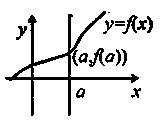
\includegraphics[scale=0.75]{4_1}
    \end{minipage}

    \noindent\begin{minipage}{0.775\textwidth}\raggedright
        $\uparrow$ 2) ``$\Leftarrow$``\\
        Покажем, как построить такую функцию. Областью определения этой функции будут все $x$, для которых пересечение прямой и множества не пусто (определили $A$).\\
        Если пересечение не пусто, то для любого такого $x = a \in A$ существует единственная точка пересечения с множеством --- $(a, b)$.
    \end{minipage}
    \hfill%
    \begin{minipage}{0.2\textwidth}\raggedleft
        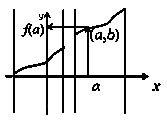
\includegraphics[scale=0.75]{4_2}
    \end{minipage}

    Т.е. мы показали, что $\forall\ a \in A \exists! b$, т.е. $\exists$ функция такая, что $b = f(a)$. Тогда точка $(a, b) = (a, f(a))$ --- это точка графика этой функции. $\downarrow$
    
    \textbf{Определение.} Назовем обратимыми такие функции $f:\ A \rightarrow B$, которые после сужения области значений $B$ до $f(A)$ становятся биекциями.

    \textbf{Теорема 2.} Функция обратима $\Leftrightarrow$, когда ее график имеет не более одной точки пересечения с любой горизонтальной прямой.

    $\uparrow$ 1) ``$\Rightarrow$`` От противного. Пусть две точки пересечения $(x_1, f(x_1))$ и $(x_2, f(x_2))$, т.е. $x_1 \neq x_2$, $f(x_1) = f(x_2) = const$.
    
    Но это противоречит обратимости функции, а именно тому, что $f$ --- вложение $(\forall x_1,\ x_2 \in A:\ x_1 \neq x_2 \Rightarrow f(x_1) \neq f(x_2))$.

    \noindent\begin{minipage}{0.65\textwidth}\raggedright
        $\uparrow$ 2) ``$\Leftarrow$``\\
        Рассмотрим прямую $y = b$, $b \in f(A)$.\\
        По условию она пересекает $\textrm{Г}_f$ в одной точке: $(a, b) = (a, f(a))$.\\
        Цепочка такая: $b \rightarrow f(a) \rightarrow a$.\\
        Тем самым задано соответствие $\forall\ b \in f(a) \exists! a$, которое определяет обратную функцию $f^{-1}$. Тогда по теореме об обратном отображении $f$ --- биекция. $\downarrow$
    \end{minipage}
    \hfill%
    \begin{minipage}{0.3\textwidth}\raggedleft
        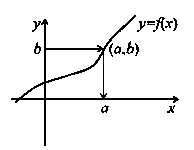
\includegraphics[scale=0.75]{4_3}
    \end{minipage}

    \textbf{Замечание.} Ответим на вопрос: как связаны между собой графики функций $f$ и $f^{-1}$?
    
    Если $f:\ a \rightarrow b$, то $f^{-1}:\ b \rightarrow a$,\\
    $(a, b) \in \textrm{Г}_f,\ (b, a) \in \textrm{Г}_f^{-1}$.

    \noindent\begin{minipage}{0.65\textwidth}\raggedright
        Заметим, что точки $(a, b),\ (a, a),\ (b, a),\ (b, b)$ на координатной плоскости являются вершинами квадрата со сторонами $\abs{b - a}$.\\
        Диагонали пересекаются под прямым углом и в точке пересечения делятся пополам.\\
        На одной из диагонали лежат точки $(a, a),\ (b, b)$. Это прямая $y = x$. Значит точки $(a, b),\ (b, a)$ другой диагонали симметричны относительно $y = x$.
    \end{minipage}
    \hfill%
    \begin{minipage}{0.3\textwidth}\raggedleft
        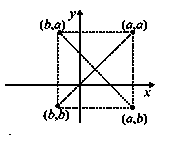
\includegraphics[scale=0.75]{4_4}
    \end{minipage}

    \textbf{Т.е. графики функций $f$ и $f^{-1}$ симметричны относительно биссектрисы первого и третьего координатных углов.}

    \textbf{Определение 2.} Функция $f:\ A \rightarrow B$ называется возрастающей (неубывающей) на множестве $A_1 \subset A$, если $\forall\ x_1, x_2 \in A_1:\ x_1 < x_2 \Rightarrow f(x_1) < f(x_2)\ (f(x_1) \leq f(x_2))$.
    
    \textbf{Определение 3.} Функция $f:\ A \rightarrow B$ называется убывающей (невозрастающей) на множестве $A_1 \subset A$, если $\forall\ x_1, x_2 \in A_1:\ x_1 < x_2 \Rightarrow f(x_1) > f(x_2)\ (f(x_1) \geq f(x_2))$.

    Обобщающее название: монотонные функции (строго монотонные и не строго монотонные).

    \textbf{Утверждение.} Покажем, что если $f(x)$ возрастает на $E$ и $g(x)$ возрастает на $E$, то их сумма $f(x) + g(x)$ возрастает на $E$.
    
    $\uparrow$ Пусть $x_1 < x_2$, тогда по условию $f(x_1) < f(x_2)$ и $g(x_1) < g(x_2)$. Отсюда $f(x_1) + g(x_1) < f(x_2) + g(x_2)$. $\downarrow$

    \textbf{Теорема 3.} Пусть $f:\ A \rightarrow B$ строго возрастает на $A$, тогда она обратима и $f^{-1}$ возрастает на $f(A)$.

    $\uparrow$ Рассмотрим $y \in f(A)$, надо показать, что прообраз существует \underline{единственный} (он есть, так как $y \in f(A)$). Это действительно так, так как если $x' \neq x$, то в силу строгого возрастания функции $f(x') < f(x)$ или $f(x) < f(x')$, т.е. $f(x') \neq f(x)$. Таким образом, определена обратная функция $f^{-1}$.
    
    Покажем, что $f^{-1}(y)$ возрастает. Пусть $y_1 < y_2$.

    Предположим, что $f^{-1}(y_1) \geq f^{-1}(y_2)$. Но $f^{-1}(y_1) = x_1$, $f^{-1}(y_2) = x_2$, а из $x_1 \geq x_2$ из строгого возрастания $f:\ y_1 = f(x_1) \geq f(x_2) = y_2$, что противоречит $y_1 < y_2$. Значит $f^{-1}(y_1) < f^{-1}(y_2)$ и $f^{-1}(y)$ возрастает. $\downarrow$

    \section{Простейшие преобразования графиков функций.}

    \textbf{1. Симметрия относительно оси \textit{OX}}

    \noindent\begin{minipage}{0.3\textwidth}
        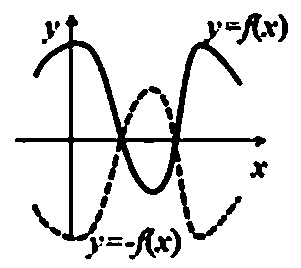
\includegraphics[scale=0.4]{4_5}
    \end{minipage}
    \hfill%
    \begin{minipage}{0.6\textwidth}\raggedright
        $(x, y) \rightarrow (x, -y)$,\\
        $\textrm{Г}_f = \{(x, f(x))\} \rightarrow \textrm{Г}_g = \{(x, -f(x))\}$, т.е.\\
        $g:\ x \rightarrow -f(x)$ и $g(x) = -f(x)$\\
        При симметрии относительно оси \textit{OX} $\textrm{Г}_f$ переходит в $\textrm{Г}_g$, т.е. для построения $g(x) = -f(x)$ надо отразить график функции симметрично относительно \textit{OX}.
    \end{minipage}

    \textbf{2. Симметрия относительно оси \textit{OY}}

    \noindent\begin{minipage}{0.3\textwidth}
        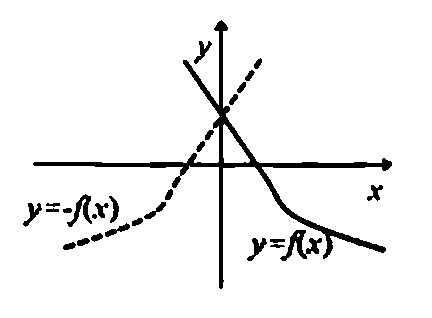
\includegraphics[scale=0.3]{4_6}
    \end{minipage}
    \hfill%
    \begin{minipage}{0.6\textwidth}\raggedright
        $(x, y) \rightarrow (-x, y)$,\\
        $\textrm{Г}_f = \{(x, f(x))\} \rightarrow \textrm{Г}_g = \{(-x, f(x))\} = \{(x', f(-x'))\}$, т.е.\\
        $g:\ x \rightarrow f(-x)$ и $g(x) = f(-x)$\\
        При симметрии относительно оси \textit{OY} $\textrm{Г}_f$ переходит в $\textrm{Г}_g$, т.е. для построения $g(x) = f(-x)$ надо отразить график функции симметрично относительно \textit{OY}.
    \end{minipage}

    \textbf{Замечание.} Отметим, что область определения функции $g:\ x \rightarrow f(-x)$ симметрична относительно нуля области определения функции $f:\ x \rightarrow f(x)$.
    
    \textbf{Определение 1.} Функция $f:\ x \rightarrow f(x)$ называется четной, если\\
    1)	$D_f$ симметрична относительно нуля;\\
    2)	$f(x) = f(-x)$.

    \textbf{3. Центральная симметрия.}
    $(x, y) \rightarrow (-x, -y)$\\
    $\textrm{Г}_f = \{(x, f(x))\} \rightarrow \textrm{Г}_g = \{(-x, -f(x))\} = \{(x', -f(-x'))\}$, т.е. $g:\ x \rightarrow -f(-x)$ и $g(x) = -f(-x)$

    При центральной симметрии $\textrm{Г}_f$ переходит в $\textrm{Г}_g$, т.е. для построения $g(x) = -f(-x)$ надо отразить график функции симметрично относительно точки $(0, 0)$.

    \textbf{Определение 2.} Функция $f:\ x \rightarrow f(x)$ называется нечетной, если\\
    1)	$D_f$ симметрична относительно нуля;\\
    2)	$f(x) = -f(x)\ (f(-x) = -f(x))$.

    % \overset{\mathrm{def}}{=}
    % \begin{figure}[h!]
    % \centering
    % 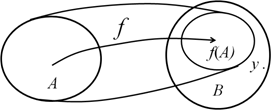
\includegraphics{2}
    % \caption{\label{fig:fig2}Разность и симметрическая разность множеств.}
    % \end{figure}

\end{document}